\documentclass[output=paper]{LSP/langsci}  
\author{Lea Schäfer, Stephanie Leser, Michael Cysouw} 
\title{Mechanisms of Dialect Imitation}
\abstract{In this article we present basic reflections into investigating the mechanisms of imitating closely related language varieties. We first conducted a survey for which speakers of German had to imitate one of five continental West Germanic lects. Furthermore, we carried out a study on imitations of Yiddish in German literature of the 19th century. In this short overview we will summarize our main results and methods from these studies, and offer some perspectives on future research in this field, which will play an important role in perceptual dialectology, psycholinguistics and even the study of language change.
}

\maketitle 
\begin{document}

\newcommand{\hai}[1]{\textsf{#1}} %für Text in Arial
\newcommand{\qu}[1]{»#1«} % >> <<
\newcommand{\quji}[1]{»#1«} %jiddische (dt.) Anführungszeichen
\newcommand{\quein}[1]{›#1‹} %einfache > <
\newcommand{\quf}[1]{\frqq#1\flqq} %franz. Anführungszeichen
\newcommand{\qufs}[1]{\frq#1\flq} %einfache franz. Anführungszeichen
\newcommand{\sem}[1]{``#1''} % 69er anführungszeichen 
   

\section{The Field of Language Imitation}\label{abstract}

Imitation is an ability that plays an important role during every process of learning.\footnote{The data of this article was presented in two posters (\citealt{schafer_language_2014} and \citealt{schafer_fictional_2014}) at \textit{Methods in Dialectologx XV} (2014) at the University of Groningen. We thank Clinton Ford, Jeffrey Pheiff and Ricarda Scherschel for checking our English. We also thank our anonymous reviewers for their useful comments.} It is one of the fundamental skills in the evolution of human communication and forms the basis of every kind of language acquisition  (e.g. \citealt{fitch_evolution_2010,hauser_language_2002,petkov_birds_2012,uzgiris_two_1981,markham_phonetic_1997,markham_listeners_1999,meltzoff_imitation_1977,meltzoff_imitative_2002}; \citealt[123]{tomasello_shared_2007}). Therefore, it is astonishing that there are barely any core linguistic works on the imitation of natural languages. The few existing studies focus mainly on phonetic and phonological questions of dialect perception; they simply use the human ability of imitation as a method for collecting data of lay concepts without questioning the mechanisms behind dialect imitation (e.\,g. \cite{segerup_imitation_1999}; \cite{siegel_second_2010}; \cite{adank_imitation_2010}; \cite{purschke_imitation_2010}; \cite{babel_phonetic_2009}; \cite{neuhauser_phonetische_2012}; \cite{dossey_spontaneous_2012}). These experiments only measure isolated non-standard features. We are advocating for experiments that simulate a situation of natural language contact and an analysis of imitation data with regard to more than just one language level, we focus upon lexis, phonology, morphology and syntax and using somehow natural stimuli instead of isolated features.
   
\section{Aspects of Dialect Imitation}\label{aspects}

The imitation of closely related varieties, like dialects of one language, differs from the imitation of non-related varieties since there is a common typological ground given in the first case, while in the second case there is not. In this article only imitation of closely-related varieties is examined. In this case we assume that the imitation can be specified as an emulative imitation. Emulation is defined as an imitation of a system through another system. The imitation of a closely related language is based on manipulations of the imitators’ own system (I-language). Exploring how these manipulations are created and what conditions influence them can be investigated by the tools of modern dialectology. Using the terminology from Myers-Scotton’s (\citeyear{myers-scotton_duelling_1993}, \citeyear{myers-scotton_contact_2002}) \textit{matrix language frame model}, which was originally designed as a model for codeswitching, imitation is made using a matrix language (ML) to which structures of a target language (TL) or what the imitator thinks of as a TL-structure are applied. Used as a model for language imitation, the ML is the speaker’s own I-language, while the TL is the language to be imitated. This is basically a simple binary model of two languages playing a role, when in fact there is a grey area in defining the ML and TL; depending on the imitator’s perception, he/she can shift between his/her own orality, the TL and what the imitator thinks is the TL.


Therefore, a language imitation model should be at least ternary. Based on the imitation of natural languages, we have to consider that the imitators have a knowledge of varieties of their own language, learned either through media, which may broadcast actual regional dialect as well as medialects\footnote{Medialects, as we call it, can be defined as artificial lects that are only used in the media. There where some investigations on the influence of dialects on such medialects from TV or internet i.\,a. by \cite{kleiner_medienbairisch_2013}, \cite{androutsopoulos_intermediale_2012}, \cite{riemann_neue_2009} or \cite{mayer_mia_2009}.)} found on television, the internet or radio and their own experience (e.\,g. migration, travelling). Once imitators recognize structures of the TL, they can match those with their concepts of a dialect or medialect. It is plausible that imitators will use structures that are not native for the TL but that are native for a similar dialect or medialect. Investigating dialect imitation always involves separating what the imitators actually know about the TL from what they believe they know. In addition, other important aspects of dialect imitation we do not focus on are mutual intelligibility and lay concepts of closely related varieties, and of course the yet not quite well defined and investigated dialectological concept of \sem{salience}. We are mainly interested in how imitation can be used as a laboratory for the ML's synchronic variability and how that could represent diachronic variability and also gives hints on innovative tendencies for the future of a dialect. 

Not only can we learn from dialect imitation how imitators interact with the lects of their surroundings, but we can also learn a lot about the ML itself. While the TL delivers the forms that \textbf{could} be imitated, the ML decides what form \textbf{can} be imitated and how.  Furthermore, there are two additional interesting aspects of dialect imitation. The first is the imitator’s spoken language (orality): imitators of a dialect will produce forms of their own orality. As a result, data from dialect imitation can be used as a source of (perhaps subconscious) structures of the ML and in general of the imitator’s orality. The second is a much deeper aspect of the ML. Through emulative imitation we get a read of the ML’s variability. It is a fascinating fact that we can produce (and process) language structures that do not conform with the structures we usually  apply. This variability represents one avenue for change that the ML possesses. 

Through emulative imitation we may even learn about the diachronic variability of the ML. As Haider (\citeyear[135]{haider_poetenpidgin_2007}) shows in his analysis of a fictional language by Ernst Jandl (an Austrian poet of the 20th century), constructed languages based on a natural ML show structures known from older periods of the language or distantly related varieties. To use a simplistic picture, we can compare a structure of a certain language to a fluid with its own viscosity. Some structures are very stressed and just show little potential for variability, thus other structures have a very low stress level and allow much variation. Our idea is that this viscosity is motivated typologically and diachronically. In this particular case of dialect imitation, the imitators can produce structures or forms that are not common for their ML (and maybe not even used in the TL); thus they can fantasise about the variability of their own ML. However, these imitators will not invent structures that differ fundamenally from the potential of their own variety. For example, when it comes to imitations of closely related varieties in discourse, like fiction, film or theater, the imitators have to make sure that the intelligibility of what they want to say is guaranteed (cf. \citeyear{SchaeferDiss}). With regard to this, evidence for fantasy forms and structures can teach us about the typological variability of the ML. With the aid of dialect imitation we can see which language structures are stable and which ones are not. To what degree this synchronic variability reflects diachronic changes has yet to be verified. The diagram in figure \ref{imitationalssubtraktiveFarbmischung} represents the factors influencing dialect imitation. As we know from classical developmental psychology: \qu{In imitating, the person constructs a match between some aspect of the external world and his or her own activity} \citep[2]{uzgiris_two_1981}. With two different data sets, presented in the following paragraph, we tried figuring out which structures of emulative dialect imitation come from the imitators' language and which derive from external languages.

\begin{figure}[htbp]
 \begin{center}
 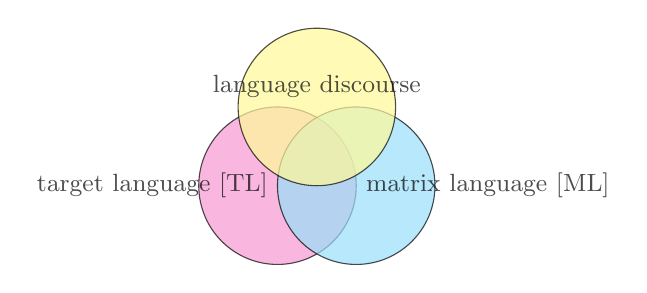
\begin{tikzpicture}
    \draw [fill=magenta!40,opacity=0.7](1,1) circle (1) node[left] {\small target language [TL]};
    \draw [fill=cyan!40,opacity=0.7](2,1) circle (1) node[right] {\small matrix language [ML]};
        \draw [fill=yellow!40,opacity=0.7] (1.5,2) circle (1) node[above] {\small language discourse};

             \end{tikzpicture}
              \caption{Sources of dialect imitation}\label{imitationalssubtraktiveFarbmischung}	
\end{center}
 \end{figure}
\FloatBarrier


Imitation of closely related varieties as we see it, is in its pure state an emulation of one dialect (TL) through an other (ML) influenced and stimulated by the ML's potential of variability which in turn is the basis of language change, which leads us to the history (and future) of the dialect that imitates (ML).

 \section{Experimental Verification}\label{experiment}
 
 
 \subsection{Internet Survey with Five West Germanic Varieties }\label{online}

To obtain a closer look at how the imitation of modern dialects works and to determine if our assumptions are correct, we designed an online survey in which a short oral story was presented to the participants. The story itself is willed with several linguistic variables; especially morpho-syntactic features like relative particles, verb-second, pronouns, progressive-constructions, negative concord, infinitive constructions and verb clusters. The story was translated and recorded by female native speakers of the following five West Germanic varieties: Belgian Dutch (BD), Low German (Westphalian, WP), Central German (Central Hessian, CH), Upper German (Alemannic, AL) and Central Eastern Yiddish (YI). These recordings were integrated into an internet survey which was completed by German-speaking informants, who listened to one random recording of the five versions of the story accompanied by a transliteration written according to the rules of Standard German orthography (for the story and its four transliterations see section \ref{appendix}, p. \pageref{appendix}). The survey was online for the whole of April 2014 using the platform \url{https://www.soscisurvey.de/}. Using social networks and mailing lists from the University of Marburg, students and staff of the faculty were recruited.

After hearing and reading the story, the informants had to make true/false decisions about seven statements concerning the content of the story. Then the actual imitation tasks began, in which Standard German sentences were given and the participants were asked to translate them by imitating the language heard beforehand. The sentences presented were structured as follows: five of the sentences were identical to sentences in the story (e.\,g. 1a), five showed lexical similarity to those in the story (e.\,g. 1b), five showed syntactic similarity, but differed lexically from those in the story  (e.\,g. 1c) and three showed no relation to sentences in the story (e.\,g. 1d).

%LS: peinlich, aber ein packet mit dem man hier automatisch nummerierte Bsp. einladen konnte und kompatibel war, konnte nicht gefunden werden.
%%%
%%% doch
%%%
\eal
%\item [a.] 
\ex Julia backt Kuchen
 \qu{Julia bakes cake} \label{bsp1}\\
%\\ [b.] 
\ex Julia braucht Milch um einen Kuchen zu backen 
 \qu{Julia needs milk to bake cake} \label{bsp2}\\
%\item [c.] 
\ex Oli schl\"aft gerade
 \qu{Oli is sleeping} \label{bsp3}\\
%\item [d.] 
\ex Ich weiß nicht, wie sp\"at es ist \qu{I do not know what time it is} \label{bsp4}\\
\zl

In addition, the informants were asked to judge their comprehension of the language of the recording and to identify the language by name. Furthermore,  the informants answered questions about their social background (e.\,g. age, gender, native language(s), education, place of longest residence). Over 600 participants completed the survey. Unfortunately, most of the German informants came from western Germany and hardly any from the East. So we can not make any dia\-topic assumptions on the whole of the German language area.

The following results are based on a sample of 353 completed questionnaires that rated themselves as non-native speakers of the heard dialect. The distribution is as follows: 61 informants imitate BD, 85 imitate WP, 84 CH, 62 AL, and 61 YI. 100 of the participants identified themselves as male, the rest as female. The average age of the participants (if trustable) is 47. The selected participants where all German native speaker and non-bilingual. 76\% (269) of the informants stated the act of imitation as \qu{difficult}, 22\% (76) as \qu{feasible} and only 2\% (7) as \qu{easy}. This does not agree with the self-assessment of the informants' understanding of the story. Following them, the understanding of the German dialects was rela\-tively good. On a scale from 1 (understand nothing) to 100 (understand everything), the hearers of WP, CH and AL rate their average all with 96 points (with a standard deviation of the WP data of 10, CH 11 and AL 8). BD was rated with a high standard deviation of 19 with 77 points as understandable. The Yiddish recording received the worst understanding. According to the self-assessment it only achieved 67 points in average. Here we find a huge standard deviation of 24.

For further analysis, we used an alignment tool that divides the relevant structures (e.g. phonetic/phonological segments or larger units, like orthographic words) into different columns so that they can be compared with one another (cf. \cite{mayer_language_2012}). Our data was aligned at four language levels: syntax, lexis, morphology, phonology (or rather its orthographic representation). With the help of this alignment, we determined that there are four possible imitation strategies based on the empirical data:
 
\begin{itemize}
\item [(1)] A form can represent the correct form of the TL (\textit{follow}), which means that the imitation of the TL was successful.
 For example, this can be seen in the correct imitation of the Central Hessian vokal in (CH) \textit{bis’} (Standard German \textit{b\"ose}) \qu{evil} as \textit{bis}.
 \item [(2)]  A form can represent neither a form of the TL nor of the ML (\textit{fantasy}); due to overgeneralization, interference with a third variety or made up form based on the potential variability of the ML. 
 For example, the \qu{do} (\textit{tun}-periphrasis) in the imitation of AL \textit{D Julia isch am Kuaha baha} lit. \sem{Julia is at baking cake} as \textit{Julia duat kuacha bacha} \qu{Julia does bake cake}. 
  \item [(3)] The imitator ignores the form of the TL and uses the ML (\textit{ignore}), means that a feature just follows the given standard language (in our case German); we do not imply any conscious act of ignoring.
  For example, an imitator does not produce the anaptyxis given in the Low German (WP) story as \textit{k\"ucket} $\to$ \textit{k\"uckt}
   \item [(4)] Due to the closeness of the TL and ML it is possible that a form could represent either language, in which case we cannot decide if this is a product of the imitation (like 1) or if it is an ignored form (like 3) (\textit{default}). As a very simple example the presented Central German (CH) form \textit{steht} \qu{stays} is equivalent with the Standard German form.
 \end{itemize}
  
In sum, the imitations were predominately (80\%) correct, i.\,e. cases in which we find the strategies (1) or (4). We compared the aligned data from all of the lects with the four imitation strategies (cf. figure \ref{alignment1}). The distribution of the aligned features shows groups that are more easily accessed by certain strategies than others. For example, in figure \ref{alignment1} the phonological analysis of one sentence reveals that there is more variation in vowels than in consonants and that the onset is more stable than the nucleus and the coda. Here we see aspects of variability and stativity that can be measured by emulative imitation data. Additional domains with vast variability can be seen as easily accessible for language change.

\begin{figure}[h!]
\centering

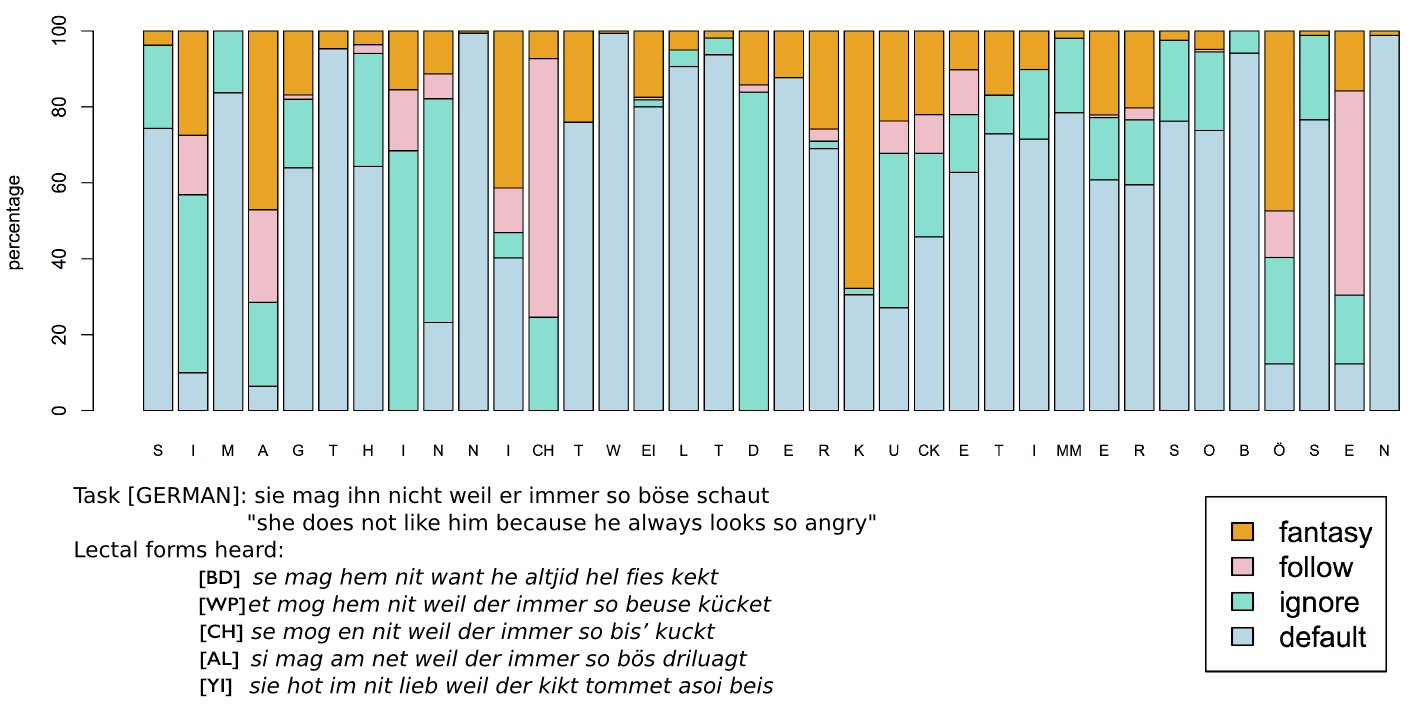
\includegraphics[width=\textwidth]{illustrations/schaf_etal_fig2}% graphics black/white???
\caption{\label{alignment1}Orthographic/phonological alignment for one sentence (all varieties)}
	\end{figure}
\FloatBarrier

Illustrating the influences of language perception, lay concepts and the imitators’ own orality we will take a closer look into the lexico-syntactic structure of pronominal adverbs. The short pronoun doubling construction (\textit{\underline{dadavon} ist Julia nicht begeistert} \qu{Julia is not excited about that} lit. \sem{\underline{therethereabout} Julia is not excited}) that was given in the Central Hessian TL was reproduced by 43\% of the imitators (like in 2a), while the stranding construction (\textit{\underline{da} ist Julia nicht begeistert \underline{von}} lit. \sem{\underline{there} is Julia not excited \underline{about}}) given in the Low German (2b) and Belgian Dutch (2c) recordings occurred in only  6\% and 3\% of the imitations of those languages, respectively (e.\,g. figure \ref{diagramdadavon}).  It is remarkable that we find the short pronoun doubling solely in the imitations of Central Hessian, where it is used in the recording. However, we do find the doubling construction in some isolated imitations of 10\% of the Alemannic variety but not in imitations of dialects that do not double their adverbs. In the case of the few instances of short pronoun doubling in the imitations of Alemannic (2d), it has to be considered that this construction is generally possible in this dialect area (e.\,g. \cite{fleischer_syntax_2002}; \cite[Round 1 Questions 11, 12; Round 2 Question 21]{ADA}), but was not used by the native speaker that translated the text into her dialect and recorded it. Here we can find an example of the influence of external factors on the imitators’ knowledge which is based on their orality or/and lay concepts.

%(2)
%\begin{enumerate} 
%\item [a.] 
\eal
\ex \textit{dadafo is Julia nit begeisderd} (Imitation of CH) \label{davon1}
%\item [b.] 
\ex \textit{Do is Julia net begeistert von} (Imitation of WP) 
%\item [c.] 
\ex \textit{da is julia net begeistered von} (Imitation of BD) 
%\item [d.] 
\ex \textit{Dodefo isch s Juli net begeischtert} (Imitation of AL)
\zl
%\end{enumerate}

\begin{figure}[h!]
\centering
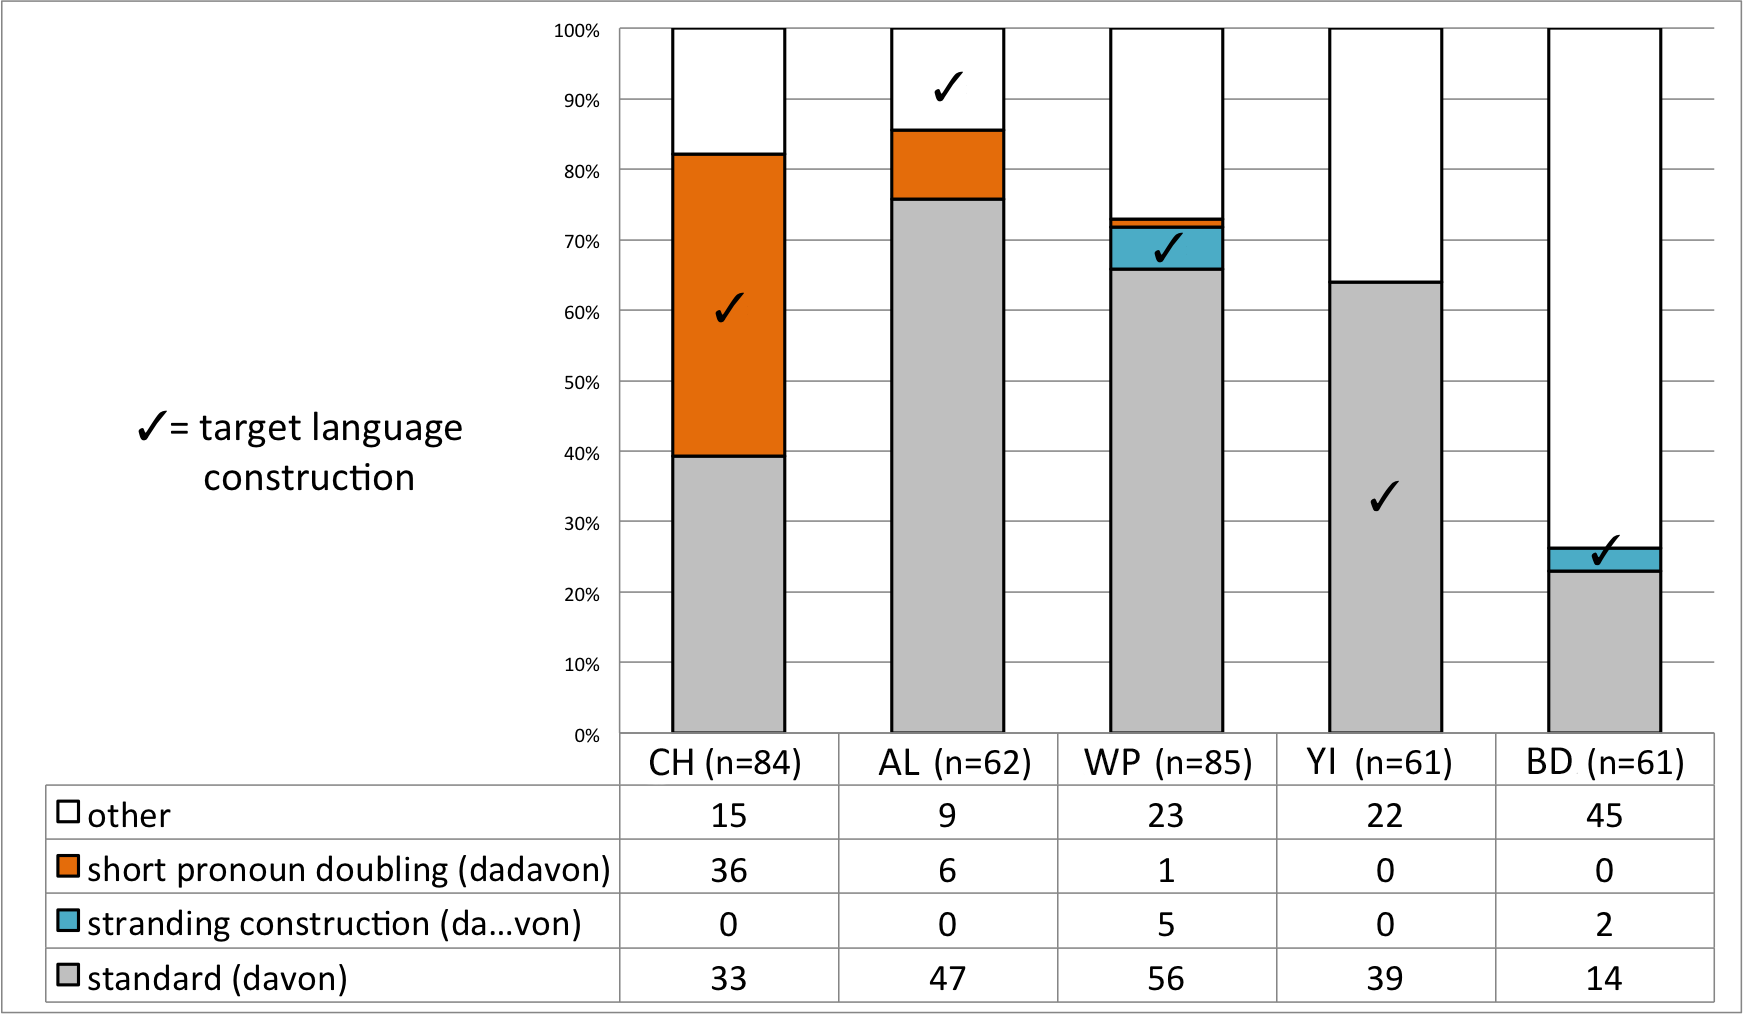
\includegraphics[scale=0.42]{illustrations/schaf_etal_fig3}% graphics black/white???
\caption{\label{diagramdadavon} Pronominal adverbs in dialect imitations (all varieties)}
	\end{figure}
\FloatBarrier


To stick with the phenomenon of pronominal adverb constructions, we can see in the maps of figure \ref{diagramdadavonhessen} the imitations of pronominal adverb constructions by our Hessian informants. Speakers from Hesse have nearly no trouble producing the construction given in the Hessian recording (\textit{dadavon}). But when it comes to other less common constructions, Hessian imitators  scarcely imitate and just keep the structure in its Standard German form (\textit{davon}). The diatopic distribution of the correctly imitated forms of pronominal adverb constructions also fits with the diatopic distribution of this phenomenon in Hessian colloquial speech where the doubling construction is common (cf. \cite{leser_zum_2012}; \cite[Round 1 Questions 11, 12; Round 2 Question 21]{ADA}). Furthermore, this picture could be caused by the factor of markedness: The pronoun doubling may stand out more than the stranding because it is a simple reduplicative construction while the stranding is just a splitting of the Standard German form. The doubling construction \textit{dadavon} compared to the Standard German \textit{davon} simply represents an increase of morphological material, while stranding \textit{da … von} is not marked by a rise or decline of material. The latter is simply a usage of the German sentence bracket (\textit{Satzklammer}).  The stranding \textit{da … von} is common in the northern German vernacular and began  entering Standard German. In the course of  doubling, we deal with the derivational phenomenon of reduplication, whereas the stranding is a syntactic feature. This difference leads us to the question of whether syntactic structures play a less important role for lay concepts than lexical-morphological do.

\begin{figure}[h!]
\centering
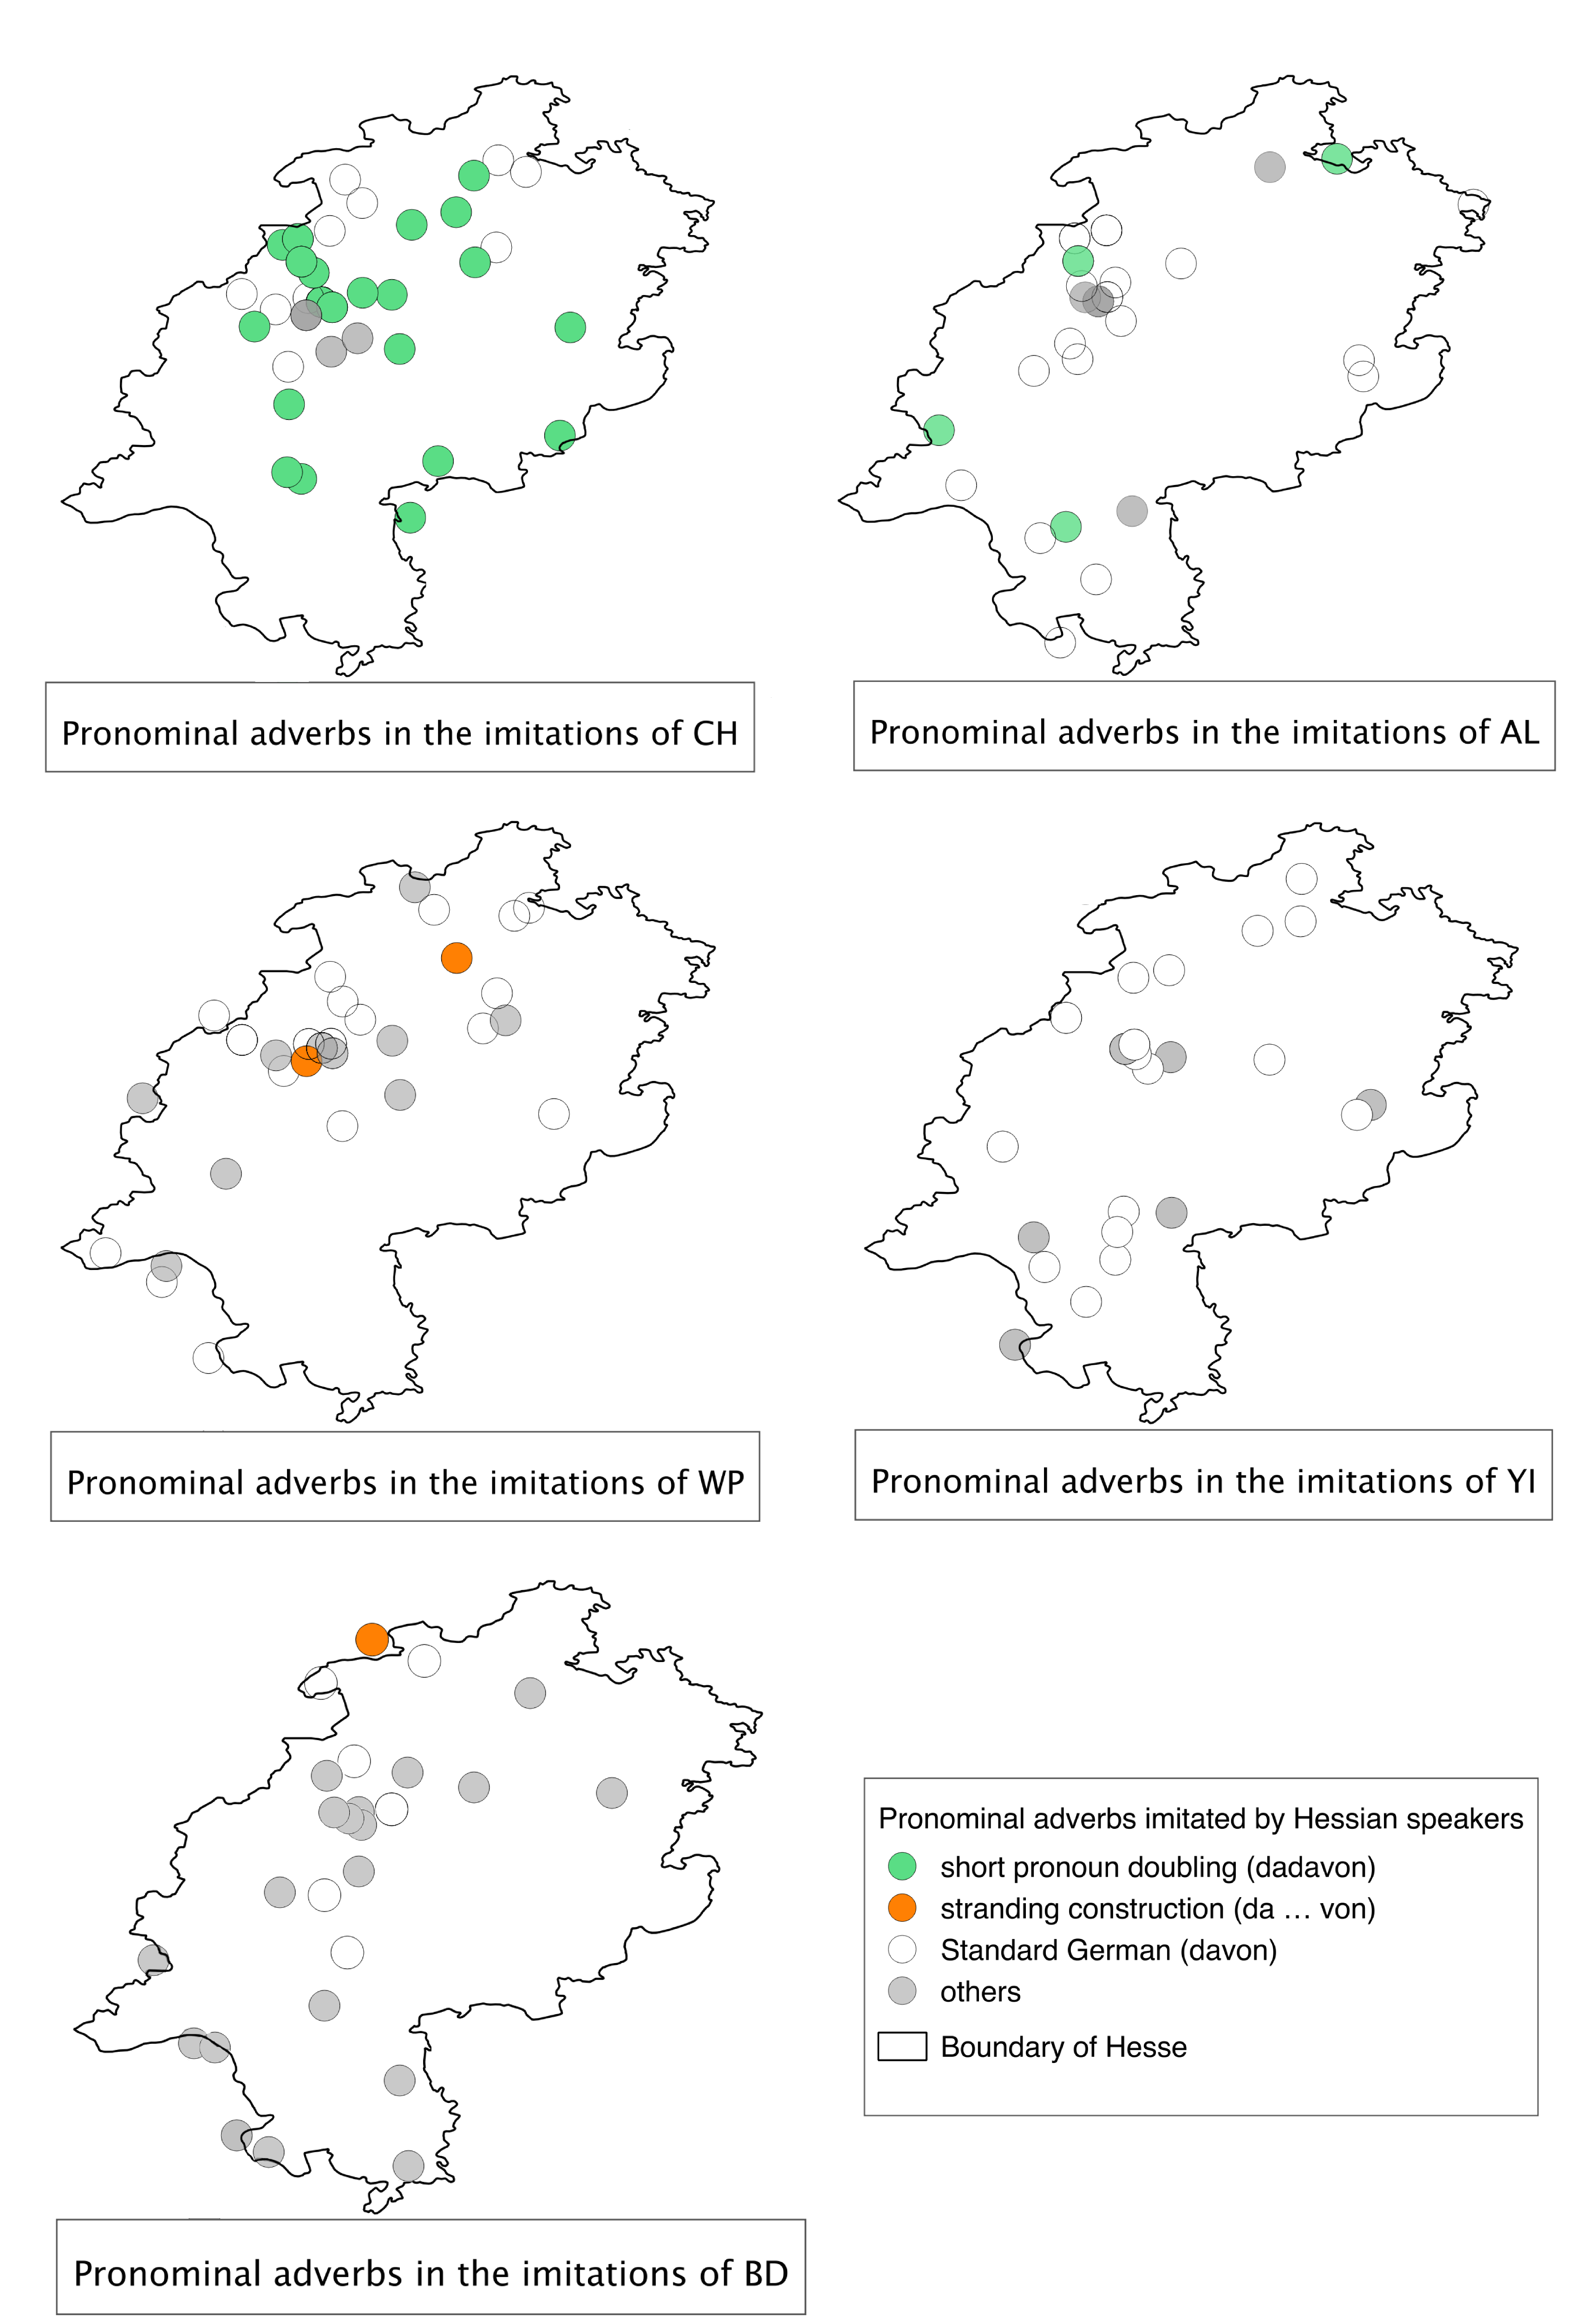
\includegraphics[scale=0.49]{illustrations/schaf_etal_fig4}% graphics black/white???
		\caption{\label{diagramdadavonhessen} Pronominal adverbs imitated by Hessian speakers (all varieties)}
	\end{figure}
%\FloatBarrier
 
	
\subsection{Corpus Study on Fictional Yiddish}\label{fiyi}
 
The second data set for language imitation dates to the 18th and the 19th century. In this period, it became fashionable in German fiction – mostly in theater plays – to mark Jewish characters via speech (cf. \cite{richter_sprache_1995}). Besides physical features (nose, beard, clothes) and ethical features (greed, incest, dishonesty), using \textit{typical Jewish} language is one strategy for evoking anti-Semitic stereotypes.
  Until the early 20th century, the vernacular of Jews in German speaking countries was  Western Yiddish. During the 19th century Western Yiddish was given up in favor of German. In contrast to Eastern Yiddish, which is still a vivid Germanic variety, Western Yiddish is not spoken anymore. The fictional adaptations of the Western Yiddish language in German literature, dating back to the 18th and 19th century, can be interpreted as an effect of the language discourse on that variety happened in that period that promoted the language death of Western Yiddish.
   As worked out by Sch\"afer (\citeyear{SchaeferDiss}) in detail, these speech styles are imitations of the Western Yiddish variety spoken in Germany, Austria,  Switzerland and  Alsace. These imitations contain many idiosyncratic structures known from Yiddish varieties, such as the merger of Middle High German /ei/ and /ou/ > /a:/. Yiddish acts here as a medialect that we will call \qu{fictional Yiddish} (fiYi) following Richters (\citeyear{richter_sprache_1995}) German term \qu{Literaturjiddisch}. To be precise, Modern Yiddish is not a dialect of German, but it is one of High German’s closest varieties. In the 18th and 19th century it was part of the German dialect continuum. We can assume that Western Yiddish was perceived as a High German variety in that period; thus fiYi is a result of a closely related variety imitation.

The research corpus on fiYi is based on 53 texts of Christian authorship with at most two sources per every 5–year-interval from 1711 to 1948. Through a descriptive and qualitative analysis of the texts, 56 grammatical elements that differ from New High German were highlighted. These fiYi elements, which were observable at all linguistic levels (lexis, phonology, morphology, syntax), were then compared with data from Western and Eastern Yiddish and German dialects of the late 19th century (based on the survey by Georg Wenker, see \cite{wenker_schriften_2013}).\\
This comparison established that all (!) 56 elements were common forms in West Germanic varieties and most of them represent forms known from Yiddish varieties. There is not a single instance of fantasy structures in the entire fiYi corpus that does not exist in a Germanic lect. Although texts from the 18th and 19th century fiYi bring together forms we would never find in a natural language. Figure \ref{RplotWJOJALLE} shows the cluster analysis of all elements used in the 53 sources plus ten fictional texts from Jewish authors from 19th century and seven sources of texts from the 21th century\footnote{The acronyms stand for the single sources (cf. \cite{SchaeferDiss}) and data from Eastern and Western Yiddish} the forms are all hypothetically feasible for a West Germanic variety. Sources of fiYi build a whole main-cluster, while the Yiddish languages build their own cluster. This evidence thus strengthens our theory that emulative imitation happens only within the bounds of its ML’s typological possibilities.
 
 \begin{figure}[h!]
%\centering
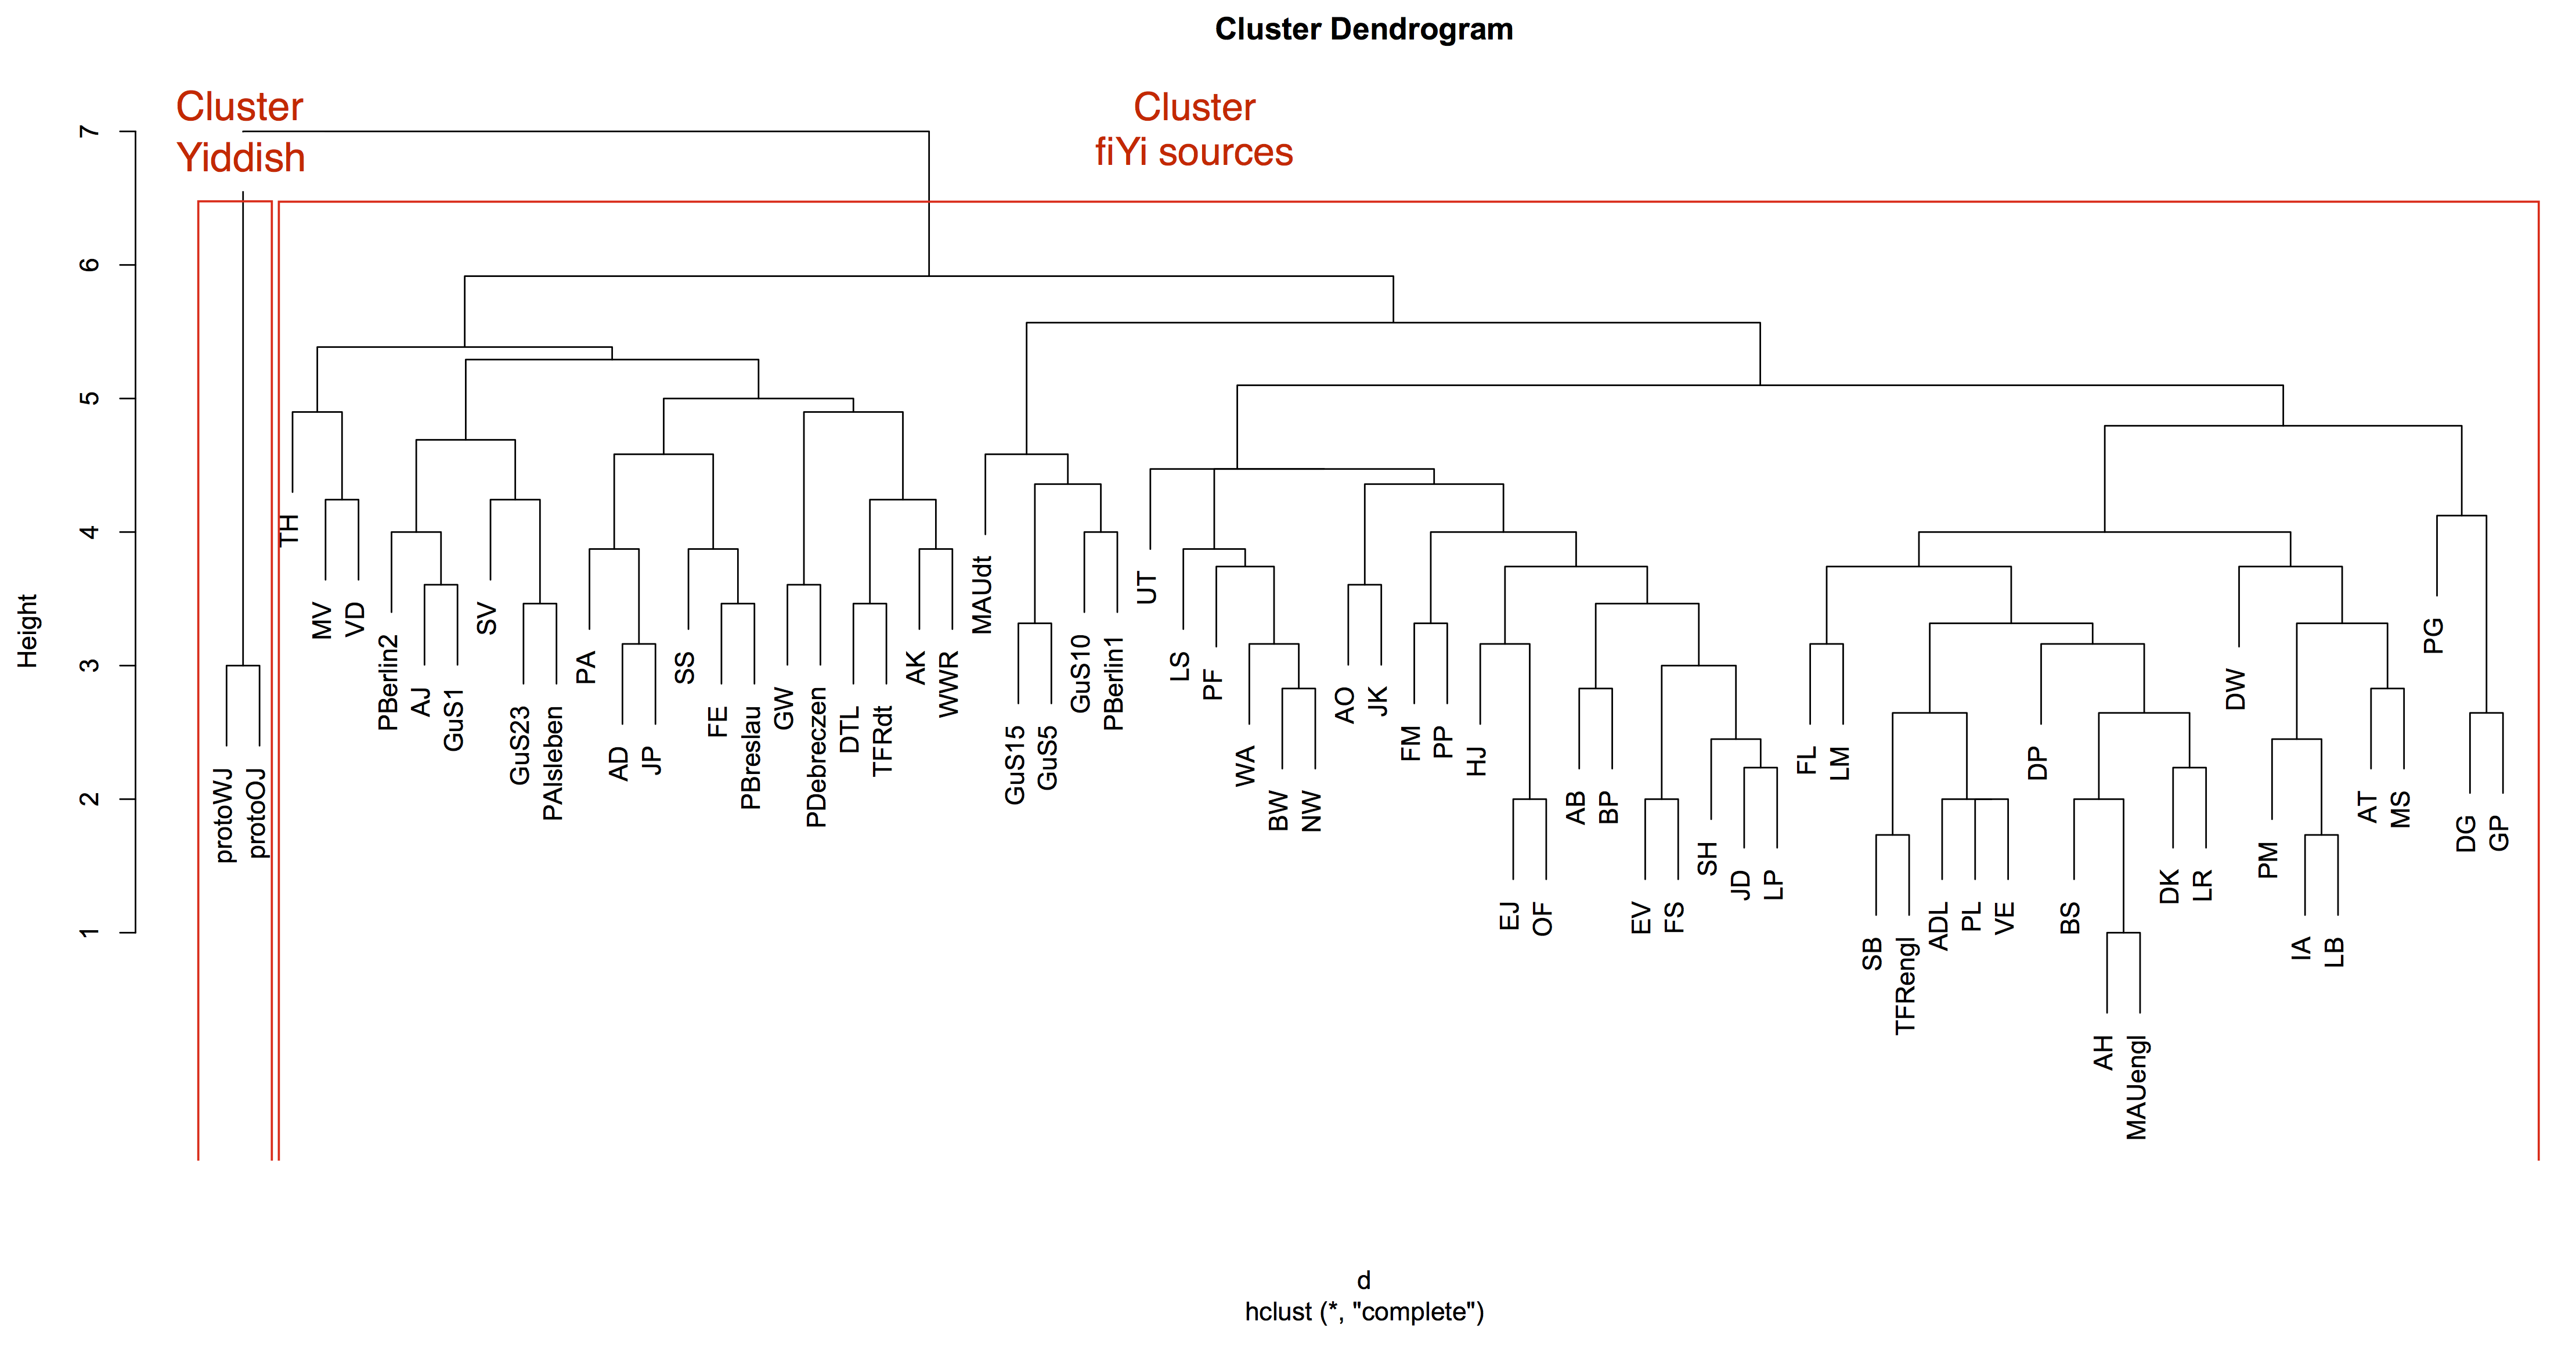
\includegraphics[width=\textwidth]{illustrations/schaf_etal_fig5}% graphics black/white???
		\caption{\label{RplotWJOJALLE} Ward-cluster of fiYi sources compared to Eastern and Western Yiddish}
	\end{figure}
\FloatBarrier
  
 \section{Outlook}\label{outlook}

In this paper, we have presented some data and a number of hypotheses and presumptions on the mechanisms of dialect imitation. We emphasize that imitation of closely related varieties  show some hidden structures of the ML that may explain to former and future changes that language did or will do.  Beyond this survey, further investigations should focus on other important attributes of language imitation, such as regional influences of the imitators’ lects, conscious versus unconscious structures used in imitation and the training curve developed during repeated imitation. We would also like to propose that those investigating dialect imitations cooperate with experts in psychology, particularly psycholinguistics, in order to benefit from their knowledge of imitation. In addition to this, there is a need for expanding the West Germanic focus of this study to include other language groups in order to determine whether the isolated mechanisms of dialect imitation can be generalized or not.

\section{Appendix}\label{appendix}

The presented story in its four translations as they where presented in the internet survey:

\small{
\noindent\textbf{Hessian [CH]}\\
Die Julia steht in der Kisch un is am Kuche backe.\\
Do merkt se, dass se f\"ur den Kuche, den se backe will, ach Milsch brauch.\\
Se kuckt nooch und stellt fest, dass se kah Milsch mehr hot. \\
‘S is Sonndach un die Gesch\"afte hon zou.\\
Also will se ihren Freund Max freje, ob der noch Milsch hot.\\
Do f\"allt er ober in, dass der Max gesagt hot, er tet ‘s Wochenende fott foan.\\
Also versucht se ’s bei der Frau Hirsch ihrer Nochbursche.\\
Die hot ober ach kah Milsch un schickt Julia bei den Herr Weiss.\\
Dodofo is se gornit begeistert, weil der immer so bis’ kuckt.\\
Ober se versuchts trotzdem.\\
Se kloppt oh sei Tir un seit, se br\"auch Milsch im e Kuche ze backe.\\
Un wer het des gedocht, der Herr Weiss hot Milsch un is fruh, dass er der Julia helfe kann.\\
Julia b\"ackt de Kuche un bringt dem Herr Weiss a gruß Stick.\\


\noindent\textbf{Yiddish [YI]}\\
Julia steiht in Kich un backt a Kichn.\\
Demolt bamerkt sie, ass sie badarf Milich farn Kichn, wos sie will backen.\\
Sie git a Kik un bamerkt, ass sie hot nischt kein Milich.\\
Es is Sunntig un die Kromen sennen farmacht.\\
Geiht sie freign ihr Freind Max, oib er hot efscher a bisl Milich far ihr.\\
Demolt gedenkt sie, ass Max hot ihr derzeilt, ass er will awekfuhrn dem Sof-Woch.\\
Geiht sie zu Frau Hirschn, ihr Schochente.\\
Jene hot oich nischt kein Milich un schickt sie zu Herr Weissn.\\
Derfin is Julia nischt bageistert, weil der kikt tommet asoi beiß.\\
Aber fundestwegen geiht sie.\\
Sie klappt un in der Tir seiner un sugt, as sie badarf Milich z' backen a Kichn.\\
'n take, wer wollt sich af dem gericht, Herr Weiss hot Milich un is glicklech ass er kenn ihr helfen.\\
Julia backt dem Kichen un brengt Herr Weissn a grois Stick.\\


\noindent\textbf{Low German [WP]}\\ 
Et Julia steiht in der K\"ucke un is an Koken backen.\\
Da merket et, f\"or den Koken, den backen will, nach Milk broket.\\
Et k\"ucket no un stellt fest, dat et keine Milk mehr do is.\\
Et is Sundach un die Jesch\"afte han to.\\
Also willt se em Freund Max frochen, of der noch welke het.\\
Dann f\"allt ‘n aber in, dat Max en vertallt h\"at, he w\"or am Wekenenne wech fahren.\\
Also fors\"oket et bi Frau Hirsch der Nachbarin.\\
Die het aber auch kinne Milk un schicket et Julia tu Herr Weiss.\\
Do is et nit begeistert von, weil der immer so beuse k\"ucket.\\
Aber et vers\"oket et trotzdem.\\
Et kloppet an sine D\"ore un seiet, dat et Milk brucket um en Koken to backen.\\
Un we hedet det jedacht, der Herr Weiss het Milk un freuet sik det he dem Julia helfen kann.\\
Julia bicket den Koken un brenget Herrn Weiss ‘n grautet St\"ucke.\\

\noindent\textbf{Belgian Dutch [BD]}\\
Julia is en de K\"oken un backt en Tart.\\
Da merkt se op, dat se vor de Tart, die se will backen, noch Milk nodich heft.\\
Se kontruliert en merkt op, dat er keen Milk mehr is.\\
H\"ot is Sundach un die Winkel sen dicht.\\
Des wil se haar Friend Max freign of he er noch heeft.\\
Dan schoot het er te binnen, dat Max haar verteeltede, dat he dat Weekend wech ching sein.\\
D\"us probiert se h\"ut be mer Frau Hirsch, her B\"urfrau.\\
Ma se heft ok keen Milk en st\"urt Julia nach min Herr Weiss.\\
Da is se nit blei um wat he altjid hel fies kekt, ma se probert het doch.\\
Se kloppt op de D\"ur en secht, dat se Mild nodich heeft om Taart te backen. \\
Wi het dat jedeicht, min Herr Weiss heft Milk un is blee dat er Julia heft k\"onne helpe.\\
Julia backt de Tart en brengt min Herr Weiss er en grot St\"uck von.\\

\noindent\textbf{Upper German [AL]}\\
D Julia isch in dr Kuhi am Kuaha baha.\\
Do merkt si, dass f\"ur an Kuaha, wo si am baha isch, noch a Milch fehlt.\\
Sie luagt nooch und sacht, dass ka Milch mer do isch.\\
Es isch Sunntig und Gsch\"after hon zua.\\
Drum goht si ihr Freund dr Max froga, ob er noch ane hot.\\
Denn fallt ira aber i, dass dr Max ira verz\"ahlt hot, er tei am Wochanende wegfahra.\\
Drum probiert sies bei dr Frau Hirsch irer Nachb\"urin.\\
Dia hot o ka Milch und schickt d Julia zum Herr Weiss.\\
Vo dem isch d Julia net begeischtert, weil der immer so b\"os driluagt.\\
Aber sie probierts trotzdem.\\
Sie klopft bei ihm an dr T\"ur und set dass sie Milch brucht zum Kuacha bacha.\\
Wer het des denkt, dr Herr Weiss hot Milch und freut sich, dass er ihra helfa k\"onna hot.\\
D Julia backt dr Kuacha und bringt am Herr Weiss a großes St\"uck.\\
}

\printbibliography[heading=subbibliography,notkeyword=this]
\end{document}
